\documentclass[twoside]{book}

% Packages required by doxygen
\usepackage{fixltx2e}
\usepackage{calc}
\usepackage{doxygen}
\usepackage[export]{adjustbox} % also loads graphicx
\usepackage{graphicx}
\usepackage[utf8]{inputenc}
\usepackage{makeidx}
\usepackage{multicol}
\usepackage{multirow}
\PassOptionsToPackage{warn}{textcomp}
\usepackage{textcomp}
\usepackage[nointegrals]{wasysym}
\usepackage[table]{xcolor}

% Font selection
\usepackage[T1]{fontenc}
\usepackage[scaled=.90]{helvet}
\usepackage{courier}
\usepackage{amssymb}
\usepackage{sectsty}
\renewcommand{\familydefault}{\sfdefault}
\allsectionsfont{%
  \fontseries{bc}\selectfont%
  \color{darkgray}%
}
\renewcommand{\DoxyLabelFont}{%
  \fontseries{bc}\selectfont%
  \color{darkgray}%
}
\newcommand{\+}{\discretionary{\mbox{\scriptsize$\hookleftarrow$}}{}{}}

% Page & text layout
\usepackage{geometry}
\geometry{%
  a4paper,%
  top=2.5cm,%
  bottom=2.5cm,%
  left=2.5cm,%
  right=2.5cm%
}
\tolerance=750
\hfuzz=15pt
\hbadness=750
\setlength{\emergencystretch}{15pt}
\setlength{\parindent}{0cm}
\setlength{\parskip}{0.2cm}
\makeatletter
\renewcommand{\paragraph}{%
  \@startsection{paragraph}{4}{0ex}{-1.0ex}{1.0ex}{%
    \normalfont\normalsize\bfseries\SS@parafont%
  }%
}
\renewcommand{\subparagraph}{%
  \@startsection{subparagraph}{5}{0ex}{-1.0ex}{1.0ex}{%
    \normalfont\normalsize\bfseries\SS@subparafont%
  }%
}
\makeatother

% Headers & footers
\usepackage{fancyhdr}
\pagestyle{fancyplain}
\fancyhead[LE]{\fancyplain{}{\bfseries\thepage}}
\fancyhead[CE]{\fancyplain{}{}}
\fancyhead[RE]{\fancyplain{}{\bfseries\leftmark}}
\fancyhead[LO]{\fancyplain{}{\bfseries\rightmark}}
\fancyhead[CO]{\fancyplain{}{}}
\fancyhead[RO]{\fancyplain{}{\bfseries\thepage}}
\fancyfoot[LE]{\fancyplain{}{}}
\fancyfoot[CE]{\fancyplain{}{}}
\fancyfoot[RE]{\fancyplain{}{\bfseries\scriptsize 生成于 2015年 四月 11日 星期六 13\+:04\+:00 , 为 Simple\+Robot使用  Doxygen }}
\fancyfoot[LO]{\fancyplain{}{\bfseries\scriptsize 生成于 2015年 四月 11日 星期六 13\+:04\+:00 , 为 Simple\+Robot使用  Doxygen }}
\fancyfoot[CO]{\fancyplain{}{}}
\fancyfoot[RO]{\fancyplain{}{}}
\renewcommand{\footrulewidth}{0.4pt}
\renewcommand{\chaptermark}[1]{%
  \markboth{#1}{}%
}
\renewcommand{\sectionmark}[1]{%
  \markright{\thesection\ #1}%
}

% Indices & bibliography
\usepackage{natbib}
\usepackage[titles]{tocloft}
\setcounter{tocdepth}{3}
\setcounter{secnumdepth}{5}
\makeindex

% Hyperlinks (required, but should be loaded last)
\usepackage{ifpdf}
\ifpdf
  \usepackage[pdftex,pagebackref=true]{hyperref}
\else
  \usepackage[ps2pdf,pagebackref=true]{hyperref}
\fi
\hypersetup{%
  colorlinks=true,%
  linkcolor=blue,%
  citecolor=blue,%
  unicode%
}

% Custom commands
\newcommand{\clearemptydoublepage}{%
  \newpage{\pagestyle{empty}\cleardoublepage}%
}


%===== C O N T E N T S =====

\begin{document}

% Titlepage & ToC
\hypersetup{pageanchor=false,
             bookmarks=true,
             bookmarksnumbered=true,
             pdfencoding=unicode
            }
\pagenumbering{roman}
\begin{titlepage}
\vspace*{7cm}
\begin{center}%
{\Large Simple\+Robot \\[1ex]\large 1.\+0 }\\
\vspace*{1cm}
{\large 制作者 Doxygen 1.8.9.1}\\
\vspace*{0.5cm}
{\small 2015年 四月 11日 星期六 13:04:00}\\
\end{center}
\end{titlepage}
\clearemptydoublepage
\tableofcontents
\clearemptydoublepage
\pagenumbering{arabic}
\hypersetup{pageanchor=true}

%--- Begin generated contents ---
\chapter{待办事项列表}
\label{todo}
\hypertarget{todo}{}

\begin{DoxyRefList}
\item[\label{todo__todo000001}%
\hypertarget{todo__todo000001}{}%
成员 \hyperlink{class_s_t_l_parser_a2e559f6f91f972c9b151593604a22002}{S\+T\+L\+Parser\+:\+:confirm\+Rule} (\hyperlink{struct_s_t_l_object}{S\+T\+L\+Object} $\ast$obj)]检测\+S\+T\+L文件是否满足格式要求 
\end{DoxyRefList}
\chapter{继承关系索引}
\section{类继承关系}
此继承关系列表按字典顺序粗略的排序\+: \begin{DoxyCompactList}
\item Q\+Object\begin{DoxyCompactList}
\item \contentsline{section}{Control}{\pageref{class_control}}{}
\item \contentsline{section}{Model}{\pageref{class_model}}{}
\end{DoxyCompactList}
\item Q\+Open\+G\+L\+Functions\begin{DoxyCompactList}
\item \contentsline{section}{View}{\pageref{class_view}}{}
\end{DoxyCompactList}
\item Q\+Open\+G\+L\+Widget\begin{DoxyCompactList}
\item \contentsline{section}{View}{\pageref{class_view}}{}
\end{DoxyCompactList}
\item \contentsline{section}{Robot}{\pageref{class_robot}}{}
\item \contentsline{section}{S\+T\+L\+Object}{\pageref{struct_s_t_l_object}}{}
\item \contentsline{section}{S\+T\+L\+Parser}{\pageref{class_s_t_l_parser}}{}
\item \contentsline{section}{S\+T\+L\+Triangle}{\pageref{struct_s_t_l_triangle}}{}
\end{DoxyCompactList}

\chapter{类索引}
\section{类列表}
这里列出了所有类、结构、联合以及接口定义等,并附带简要说明\+:\begin{DoxyCompactList}
\item\contentsline{section}{\hyperlink{class_control}{Control} \\*控制类 }{\pageref{class_control}}{}
\item\contentsline{section}{\hyperlink{class_model}{Model} \\*机器人数据模型 }{\pageref{class_model}}{}
\item\contentsline{section}{\hyperlink{class_robot}{Robot} \\*机器人类 }{\pageref{class_robot}}{}
\item\contentsline{section}{\hyperlink{struct_s_t_l_object}{S\+T\+L\+Object} \\*S\+T\+L数据类 }{\pageref{struct_s_t_l_object}}{}
\item\contentsline{section}{\hyperlink{class_s_t_l_parser}{S\+T\+L\+Parser} \\*S\+T\+L解析器 }{\pageref{class_s_t_l_parser}}{}
\item\contentsline{section}{\hyperlink{struct_s_t_l_triangle}{S\+T\+L\+Triangle} \\*S\+T\+L三角面类 }{\pageref{struct_s_t_l_triangle}}{}
\item\contentsline{section}{\hyperlink{class_view}{View} \\*视图类 }{\pageref{class_view}}{}
\end{DoxyCompactList}

\chapter{类说明}
\hypertarget{class_control}{}\section{Control类 参考}
\label{class_control}\index{Control@{Control}}


控制类  




{\ttfamily \#include $<$control.\+h$>$}

类 Control 继承关系图\+:\begin{figure}[H]
\begin{center}
\leavevmode
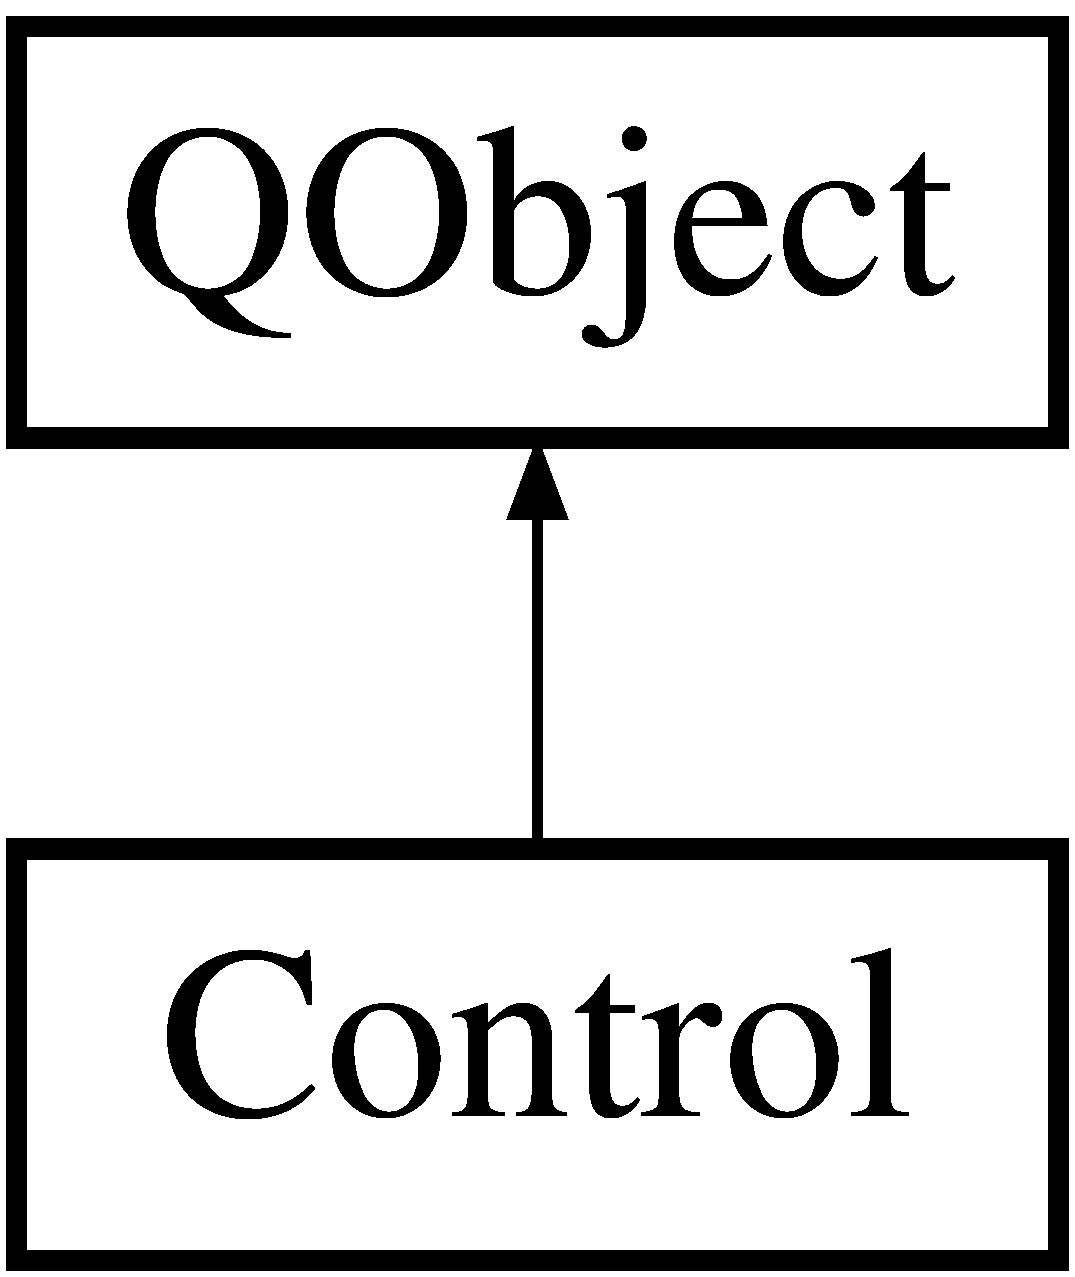
\includegraphics[height=2.000000cm]{class_control}
\end{center}
\end{figure}
\subsection*{信号}
\begin{DoxyCompactItemize}
\item 
\hypertarget{class_control_aa3dfe35b337f0342abc4aaa9b25d334a}{}void \hyperlink{class_control_aa3dfe35b337f0342abc4aaa9b25d334a}{action\+Finished} ()\label{class_control_aa3dfe35b337f0342abc4aaa9b25d334a}

\begin{DoxyCompactList}\small\item\em 动作完成信号 \end{DoxyCompactList}\end{DoxyCompactItemize}
\subsection*{Public 成员函数}
\begin{DoxyCompactItemize}
\item 
\hypertarget{class_control_aa730aeda4517f40bc48ba1e46ebded77}{}\hyperlink{class_control_aa730aeda4517f40bc48ba1e46ebded77}{Control} ()\label{class_control_aa730aeda4517f40bc48ba1e46ebded77}

\begin{DoxyCompactList}\small\item\em A constructor. \end{DoxyCompactList}\item 
\hypertarget{class_control_aedda1328c4f8b8d49bca8f0812d3bfd1}{}\hyperlink{class_control_aedda1328c4f8b8d49bca8f0812d3bfd1}{$\sim$\+Control} ()\label{class_control_aedda1328c4f8b8d49bca8f0812d3bfd1}

\begin{DoxyCompactList}\small\item\em A destructor. \end{DoxyCompactList}\item 
bool \hyperlink{class_control_ad223c63a5825a584f17a4cfc3b1b021d}{Rotate\+Master\+Abs} (float angle, float speed=-\/1, bool immediate=false)
\begin{DoxyCompactList}\small\item\em 旋转主臂到指定角度 \end{DoxyCompactList}\item 
bool \hyperlink{class_control_ada672bd88cf68c704896094e831c6712}{Rotate\+Master} (float angle, float speed=-\/1, bool immediate=false)
\begin{DoxyCompactList}\small\item\em 旋转主臂指定大小的角度 \end{DoxyCompactList}\item 
bool \hyperlink{class_control_a8639f928bd61943fc7f7a1f57b9aa544}{Rotate\+Assistant\+Abs} (float angle, float speed=-\/1, bool immediate=false)
\begin{DoxyCompactList}\small\item\em 旋转副臂到指定角度 \end{DoxyCompactList}\item 
bool \hyperlink{class_control_a1472aabfe513d8abd7e55fa665ca5ed4}{Rotate\+Assistant} (float angle, float speed=-\/1, bool immediate=false)
\begin{DoxyCompactList}\small\item\em 旋转副臂指定大小的角度 \end{DoxyCompactList}\item 
bool \hyperlink{class_control_a7a42b29c54f6bbcde494a57489fe9f70}{Rotate\+Bar\+Abs} (float angle, float speed=-\/1, bool immediate=false)
\begin{DoxyCompactList}\small\item\em 旋转工具杆到指定角度 \end{DoxyCompactList}\item 
bool \hyperlink{class_control_ae7a6809f813de5bf1ad1eaf682d572df}{Rotate\+Bar} (float angle, float speed=-\/1, bool immediate=false)
\begin{DoxyCompactList}\small\item\em 旋转工具杆指定大小的角度 \end{DoxyCompactList}\item 
bool \hyperlink{class_control_a1e089b19f49a8214e5791fa2fbd87cce}{Move\+Bar\+Abs} (float down, float speed=-\/1, bool immediate=false)
\begin{DoxyCompactList}\small\item\em 移动工具杆到指定位置 \end{DoxyCompactList}\item 
bool \hyperlink{class_control_a0e6e5b1243a21767a4707639a6536ef6}{Move\+Bar} (float down, float speed=-\/1, bool immediate=false)
\begin{DoxyCompactList}\small\item\em 移动工具杆指定大小的位移 \end{DoxyCompactList}\item 
\hypertarget{class_control_ad408f3b1eaf5b30c96600f4a299c0119}{}void \hyperlink{class_control_ad408f3b1eaf5b30c96600f4a299c0119}{Stop} ()\label{class_control_ad408f3b1eaf5b30c96600f4a299c0119}

\begin{DoxyCompactList}\small\item\em 停止运动 \end{DoxyCompactList}\item 
void \hyperlink{class_control_ab356fe0c8c30559cbeeb38d4b2c4cc1b}{set\+Model} (\hyperlink{class_model}{Model} $\ast$model)
\begin{DoxyCompactList}\small\item\em 设置数据模型 \end{DoxyCompactList}\item 
void \hyperlink{class_control_a265d02f2f3c4e5bcffab2726ae72b54c}{set\+View} (\hyperlink{class_view}{View} $\ast$view)
\begin{DoxyCompactList}\small\item\em 设置3\+D视图 \end{DoxyCompactList}\item 
void \hyperlink{class_control_adf3a4b133db05f5c0a454fc125ab4d68}{set\+Finished\+Signal} (bool open)
\begin{DoxyCompactList}\small\item\em 开关结束信号 \end{DoxyCompactList}\end{DoxyCompactItemize}
\subsection*{Public 属性}
\begin{DoxyCompactItemize}
\item 
\hypertarget{class_control_a3cfae96ae72da599e682bee89f561527}{}float \hyperlink{class_control_a3cfae96ae72da599e682bee89f561527}{internal\+Msecs}\label{class_control_a3cfae96ae72da599e682bee89f561527}

\begin{DoxyCompactList}\small\item\em 定时刷新时间 \end{DoxyCompactList}\end{DoxyCompactItemize}
\subsection*{Protected 槽}
\begin{DoxyCompactItemize}
\item 
\hypertarget{class_control_a06e70e1ef83056e2ec2925d17d1dfbde}{}void \hyperlink{class_control_a06e70e1ef83056e2ec2925d17d1dfbde}{on\+Paint\+Tick} ()\label{class_control_a06e70e1ef83056e2ec2925d17d1dfbde}

\begin{DoxyCompactList}\small\item\em 定时器中断槽 \end{DoxyCompactList}\end{DoxyCompactItemize}


\subsection{详细描述}
控制类 

\subsection{成员函数说明}
\hypertarget{class_control_a0e6e5b1243a21767a4707639a6536ef6}{}\index{Control@{Control}!Move\+Bar@{Move\+Bar}}
\index{Move\+Bar@{Move\+Bar}!Control@{Control}}
\subsubsection[{Move\+Bar}]{\setlength{\rightskip}{0pt plus 5cm}bool Control\+::\+Move\+Bar (
\begin{DoxyParamCaption}
\item[{float}]{down, }
\item[{float}]{speed = {\ttfamily -\/1}, }
\item[{bool}]{immediate = {\ttfamily false}}
\end{DoxyParamCaption}
)\hspace{0.3cm}{\ttfamily [inline]}}\label{class_control_a0e6e5b1243a21767a4707639a6536ef6}


移动工具杆指定大小的位移 


\begin{DoxyParams}{参数}
{\em down} & 位移 \\
\hline
{\em speed} & 速度(-\/1 or 1-\/100) \\
\hline
{\em immediate} & 是否立即到达 \\
\hline
\end{DoxyParams}
\hypertarget{class_control_a1e089b19f49a8214e5791fa2fbd87cce}{}\index{Control@{Control}!Move\+Bar\+Abs@{Move\+Bar\+Abs}}
\index{Move\+Bar\+Abs@{Move\+Bar\+Abs}!Control@{Control}}
\subsubsection[{Move\+Bar\+Abs}]{\setlength{\rightskip}{0pt plus 5cm}bool Control\+::\+Move\+Bar\+Abs (
\begin{DoxyParamCaption}
\item[{float}]{down, }
\item[{float}]{speed = {\ttfamily -\/1}, }
\item[{bool}]{immediate = {\ttfamily false}}
\end{DoxyParamCaption}
)\hspace{0.3cm}{\ttfamily [inline]}}\label{class_control_a1e089b19f49a8214e5791fa2fbd87cce}


移动工具杆到指定位置 


\begin{DoxyParams}{参数}
{\em down} & 位置 \\
\hline
{\em speed} & 速度(-\/1 or 1-\/100) \\
\hline
{\em immediate} & 是否立即到达 \\
\hline
\end{DoxyParams}
\hypertarget{class_control_a1472aabfe513d8abd7e55fa665ca5ed4}{}\index{Control@{Control}!Rotate\+Assistant@{Rotate\+Assistant}}
\index{Rotate\+Assistant@{Rotate\+Assistant}!Control@{Control}}
\subsubsection[{Rotate\+Assistant}]{\setlength{\rightskip}{0pt plus 5cm}bool Control\+::\+Rotate\+Assistant (
\begin{DoxyParamCaption}
\item[{float}]{angle, }
\item[{float}]{speed = {\ttfamily -\/1}, }
\item[{bool}]{immediate = {\ttfamily false}}
\end{DoxyParamCaption}
)\hspace{0.3cm}{\ttfamily [inline]}}\label{class_control_a1472aabfe513d8abd7e55fa665ca5ed4}


旋转副臂指定大小的角度 


\begin{DoxyParams}{参数}
{\em angle} & 角度 \\
\hline
{\em speed} & 速度(-\/1 or 1-\/100) \\
\hline
{\em immediate} & 是否立即到达 \\
\hline
\end{DoxyParams}
\hypertarget{class_control_a8639f928bd61943fc7f7a1f57b9aa544}{}\index{Control@{Control}!Rotate\+Assistant\+Abs@{Rotate\+Assistant\+Abs}}
\index{Rotate\+Assistant\+Abs@{Rotate\+Assistant\+Abs}!Control@{Control}}
\subsubsection[{Rotate\+Assistant\+Abs}]{\setlength{\rightskip}{0pt plus 5cm}bool Control\+::\+Rotate\+Assistant\+Abs (
\begin{DoxyParamCaption}
\item[{float}]{angle, }
\item[{float}]{speed = {\ttfamily -\/1}, }
\item[{bool}]{immediate = {\ttfamily false}}
\end{DoxyParamCaption}
)\hspace{0.3cm}{\ttfamily [inline]}}\label{class_control_a8639f928bd61943fc7f7a1f57b9aa544}


旋转副臂到指定角度 


\begin{DoxyParams}{参数}
{\em angle} & 角度 \\
\hline
{\em speed} & 速度(-\/1 or 1-\/100) \\
\hline
{\em immediate} & 是否立即到达 \\
\hline
\end{DoxyParams}
\hypertarget{class_control_ae7a6809f813de5bf1ad1eaf682d572df}{}\index{Control@{Control}!Rotate\+Bar@{Rotate\+Bar}}
\index{Rotate\+Bar@{Rotate\+Bar}!Control@{Control}}
\subsubsection[{Rotate\+Bar}]{\setlength{\rightskip}{0pt plus 5cm}bool Control\+::\+Rotate\+Bar (
\begin{DoxyParamCaption}
\item[{float}]{angle, }
\item[{float}]{speed = {\ttfamily -\/1}, }
\item[{bool}]{immediate = {\ttfamily false}}
\end{DoxyParamCaption}
)\hspace{0.3cm}{\ttfamily [inline]}}\label{class_control_ae7a6809f813de5bf1ad1eaf682d572df}


旋转工具杆指定大小的角度 


\begin{DoxyParams}{参数}
{\em angle} & 角度 \\
\hline
{\em speed} & 速度(-\/1 or 1-\/100) \\
\hline
{\em immediate} & 是否立即到达 \\
\hline
\end{DoxyParams}
\hypertarget{class_control_a7a42b29c54f6bbcde494a57489fe9f70}{}\index{Control@{Control}!Rotate\+Bar\+Abs@{Rotate\+Bar\+Abs}}
\index{Rotate\+Bar\+Abs@{Rotate\+Bar\+Abs}!Control@{Control}}
\subsubsection[{Rotate\+Bar\+Abs}]{\setlength{\rightskip}{0pt plus 5cm}bool Control\+::\+Rotate\+Bar\+Abs (
\begin{DoxyParamCaption}
\item[{float}]{angle, }
\item[{float}]{speed = {\ttfamily -\/1}, }
\item[{bool}]{immediate = {\ttfamily false}}
\end{DoxyParamCaption}
)\hspace{0.3cm}{\ttfamily [inline]}}\label{class_control_a7a42b29c54f6bbcde494a57489fe9f70}


旋转工具杆到指定角度 


\begin{DoxyParams}{参数}
{\em angle} & 角度 \\
\hline
{\em speed} & 速度(-\/1 or 1-\/100) \\
\hline
{\em immediate} & 是否立即到达 \\
\hline
\end{DoxyParams}
\hypertarget{class_control_ada672bd88cf68c704896094e831c6712}{}\index{Control@{Control}!Rotate\+Master@{Rotate\+Master}}
\index{Rotate\+Master@{Rotate\+Master}!Control@{Control}}
\subsubsection[{Rotate\+Master}]{\setlength{\rightskip}{0pt plus 5cm}bool Control\+::\+Rotate\+Master (
\begin{DoxyParamCaption}
\item[{float}]{angle, }
\item[{float}]{speed = {\ttfamily -\/1}, }
\item[{bool}]{immediate = {\ttfamily false}}
\end{DoxyParamCaption}
)\hspace{0.3cm}{\ttfamily [inline]}}\label{class_control_ada672bd88cf68c704896094e831c6712}


旋转主臂指定大小的角度 


\begin{DoxyParams}{参数}
{\em angle} & 角度 \\
\hline
{\em speed} & 速度(-\/1 or 1-\/100) \\
\hline
{\em immediate} & 是否立即到达 \\
\hline
\end{DoxyParams}
\hypertarget{class_control_ad223c63a5825a584f17a4cfc3b1b021d}{}\index{Control@{Control}!Rotate\+Master\+Abs@{Rotate\+Master\+Abs}}
\index{Rotate\+Master\+Abs@{Rotate\+Master\+Abs}!Control@{Control}}
\subsubsection[{Rotate\+Master\+Abs}]{\setlength{\rightskip}{0pt plus 5cm}bool Control\+::\+Rotate\+Master\+Abs (
\begin{DoxyParamCaption}
\item[{float}]{angle, }
\item[{float}]{speed = {\ttfamily -\/1}, }
\item[{bool}]{immediate = {\ttfamily false}}
\end{DoxyParamCaption}
)\hspace{0.3cm}{\ttfamily [inline]}}\label{class_control_ad223c63a5825a584f17a4cfc3b1b021d}


旋转主臂到指定角度 


\begin{DoxyParams}{参数}
{\em angle} & 角度 \\
\hline
{\em speed} & 速度(-\/1 or 1-\/100) \\
\hline
{\em immediate} & 是否立即到达 \\
\hline
\end{DoxyParams}
\hypertarget{class_control_adf3a4b133db05f5c0a454fc125ab4d68}{}\index{Control@{Control}!set\+Finished\+Signal@{set\+Finished\+Signal}}
\index{set\+Finished\+Signal@{set\+Finished\+Signal}!Control@{Control}}
\subsubsection[{set\+Finished\+Signal}]{\setlength{\rightskip}{0pt plus 5cm}void Control\+::set\+Finished\+Signal (
\begin{DoxyParamCaption}
\item[{bool}]{open}
\end{DoxyParamCaption}
)\hspace{0.3cm}{\ttfamily [inline]}}\label{class_control_adf3a4b133db05f5c0a454fc125ab4d68}


开关结束信号 


\begin{DoxyParams}{参数}
{\em open} & 打开结束信号? \\
\hline
\end{DoxyParams}
\hypertarget{class_control_ab356fe0c8c30559cbeeb38d4b2c4cc1b}{}\index{Control@{Control}!set\+Model@{set\+Model}}
\index{set\+Model@{set\+Model}!Control@{Control}}
\subsubsection[{set\+Model}]{\setlength{\rightskip}{0pt plus 5cm}void Control\+::set\+Model (
\begin{DoxyParamCaption}
\item[{{\bf Model} $\ast$}]{model}
\end{DoxyParamCaption}
)\hspace{0.3cm}{\ttfamily [inline]}}\label{class_control_ab356fe0c8c30559cbeeb38d4b2c4cc1b}


设置数据模型 


\begin{DoxyParams}{参数}
{\em model} & 数据模型指针 \\
\hline
\end{DoxyParams}
\hypertarget{class_control_a265d02f2f3c4e5bcffab2726ae72b54c}{}\index{Control@{Control}!set\+View@{set\+View}}
\index{set\+View@{set\+View}!Control@{Control}}
\subsubsection[{set\+View}]{\setlength{\rightskip}{0pt plus 5cm}void Control\+::set\+View (
\begin{DoxyParamCaption}
\item[{{\bf View} $\ast$}]{view}
\end{DoxyParamCaption}
)\hspace{0.3cm}{\ttfamily [inline]}}\label{class_control_a265d02f2f3c4e5bcffab2726ae72b54c}


设置3\+D视图 


\begin{DoxyParams}{参数}
{\em view} & 3\+D视图指针 \\
\hline
\end{DoxyParams}


该类的文档由以下文件生成\+:\begin{DoxyCompactItemize}
\item 
/\+Users/firemiles/\+Developer/\+Open\+G\+L/\+Simple\+Robot/robot/control.\+h\item 
/\+Users/firemiles/\+Developer/\+Open\+G\+L/\+Simple\+Robot/robot/control.\+cpp\end{DoxyCompactItemize}

\hypertarget{class_model}{}\section{Model类 参考}
\label{class_model}\index{Model@{Model}}


机器人数据模型  




{\ttfamily \#include $<$model.\+h$>$}

类 Model 继承关系图\+:\begin{figure}[H]
\begin{center}
\leavevmode
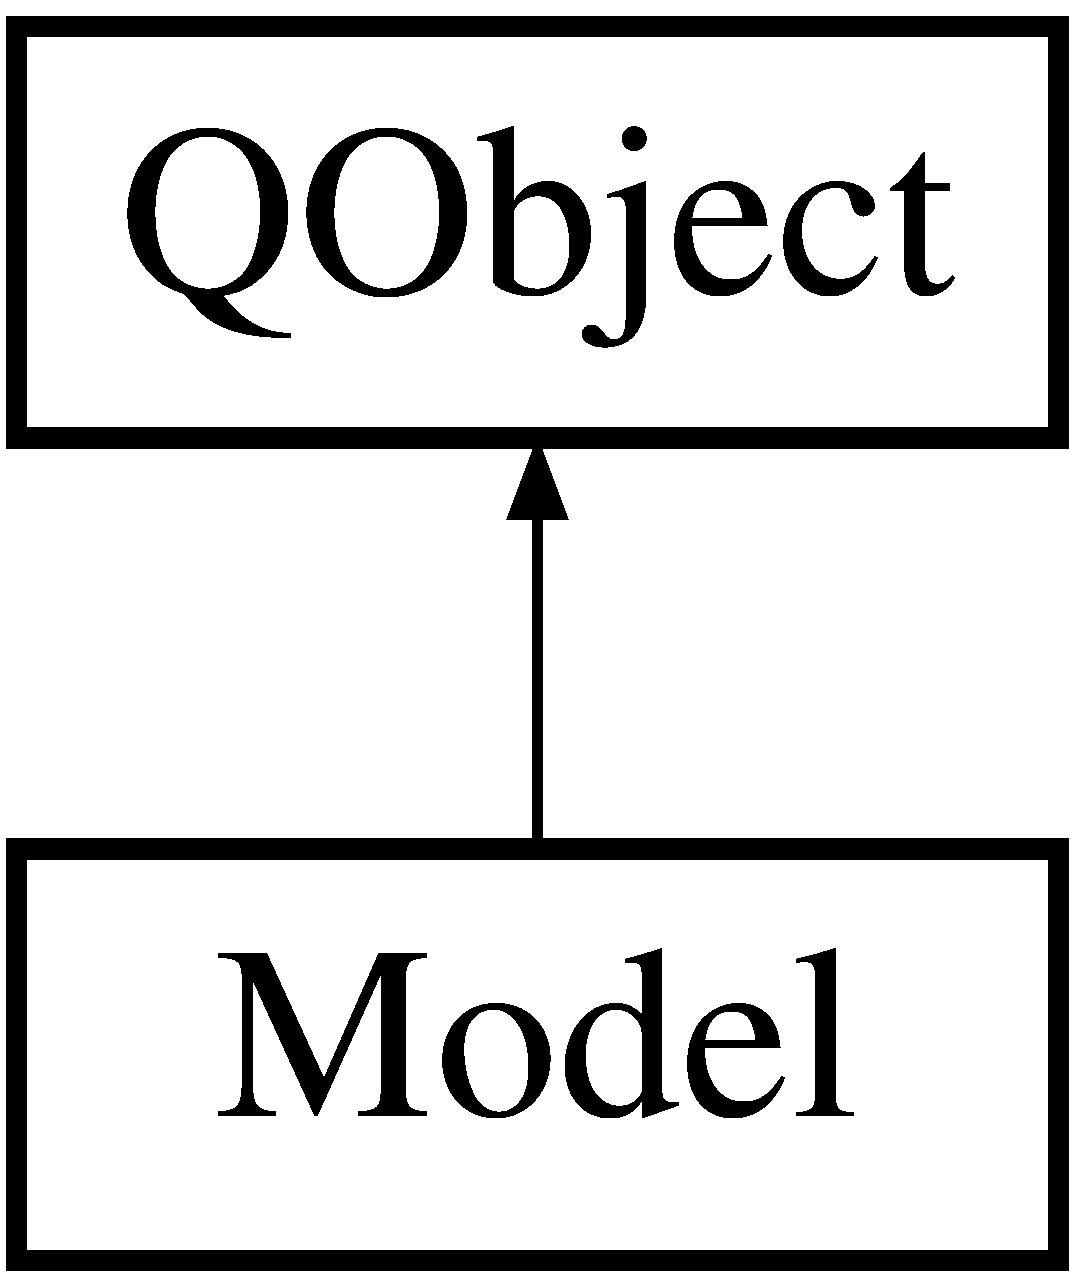
\includegraphics[height=2.000000cm]{class_model}
\end{center}
\end{figure}
\subsection*{Public 类型}
\begin{DoxyCompactItemize}
\item 
\hypertarget{class_model_a639d17254535dbda93359bed8722e6c7}{}enum \hyperlink{class_model_a639d17254535dbda93359bed8722e6c7}{Action\+Type} \{ {\bfseries M\+A\+S\+T\+E\+R\+\_\+\+R\+O\+T\+A\+T\+E} =0, 
{\bfseries A\+S\+S\+I\+S\+T\+A\+N\+T\+\_\+\+R\+O\+T\+A\+T\+E} =1, 
{\bfseries B\+A\+R\+\_\+\+R\+O\+T\+A\+T\+E} =2, 
{\bfseries B\+A\+R\+\_\+\+M\+O\+V\+E} =3
 \}\label{class_model_a639d17254535dbda93359bed8722e6c7}

\begin{DoxyCompactList}\small\item\em 动作类型 \end{DoxyCompactList}\item 
\hypertarget{class_model_a997cd2b5b12b228bfbcdc1829e75352b}{}enum \hyperlink{class_model_a997cd2b5b12b228bfbcdc1829e75352b}{Model\+Type} \{ {\bfseries B\+A\+S\+E} =0, 
{\bfseries M\+A\+S\+T\+E\+R} =1, 
{\bfseries A\+S\+S\+I\+S\+T\+A\+N\+T} =2, 
{\bfseries B\+A\+R} =3
 \}\label{class_model_a997cd2b5b12b228bfbcdc1829e75352b}

\begin{DoxyCompactList}\small\item\em 模型部位 \end{DoxyCompactList}\end{DoxyCompactItemize}
\subsection*{Public 成员函数}
\begin{DoxyCompactItemize}
\item 
\hypertarget{class_model_ae3b375de5f6df4faf74a95d64748e048}{}\hyperlink{class_model_ae3b375de5f6df4faf74a95d64748e048}{Model} ()\label{class_model_ae3b375de5f6df4faf74a95d64748e048}

\begin{DoxyCompactList}\small\item\em A constructor. \end{DoxyCompactList}\item 
\hypertarget{class_model_ad6ebd2062a0b823db841a0b88baac4c0}{}\hyperlink{class_model_ad6ebd2062a0b823db841a0b88baac4c0}{$\sim$\+Model} ()\label{class_model_ad6ebd2062a0b823db841a0b88baac4c0}

\begin{DoxyCompactList}\small\item\em A destructor. \end{DoxyCompactList}\item 
\hypertarget{class_model_a7277e94b38e6f196f34499a3e9996348}{}const Q\+Vector$<$ float $>$ \& \hyperlink{class_model_a7277e94b38e6f196f34499a3e9996348}{get\+Model\+Verteces} () const \label{class_model_a7277e94b38e6f196f34499a3e9996348}

\begin{DoxyCompactList}\small\item\em 获取模型顶点 \end{DoxyCompactList}\item 
\hypertarget{class_model_ada3d4d3d12d9b59be940584df5231cf9}{}const Q\+Vector$<$ float $>$ \& \hyperlink{class_model_ada3d4d3d12d9b59be940584df5231cf9}{get\+Model\+Normals} () const \label{class_model_ada3d4d3d12d9b59be940584df5231cf9}

\begin{DoxyCompactList}\small\item\em 获取模型法向量 \end{DoxyCompactList}\item 
\hypertarget{class_model_afd605efc0857e7b3789981585e904196}{}unsigned int \hyperlink{class_model_afd605efc0857e7b3789981585e904196}{get\+Model\+Verteces\+Num} (\hyperlink{class_model_a997cd2b5b12b228bfbcdc1829e75352b}{Model\+Type} model\+Type) const \label{class_model_afd605efc0857e7b3789981585e904196}

\begin{DoxyCompactList}\small\item\em 获取模型顶点数目 \end{DoxyCompactList}\item 
\hypertarget{class_model_a4f3fd5b3fc2b7eb384a43c5467dd61fd}{}void \hyperlink{class_model_a4f3fd5b3fc2b7eb384a43c5467dd61fd}{reset\+Value} ()\label{class_model_a4f3fd5b3fc2b7eb384a43c5467dd61fd}

\begin{DoxyCompactList}\small\item\em 重置机器人位置 \end{DoxyCompactList}\item 
\hypertarget{class_model_a6481ca1940a8fc95128fc599f984b53b}{}float \hyperlink{class_model_a6481ca1940a8fc95128fc599f984b53b}{Calc\+Cur\+Value} (\hyperlink{class_model_a639d17254535dbda93359bed8722e6c7}{Action\+Type} action\+Type, float spend\+Seconds, bool $\ast$reached)\label{class_model_a6481ca1940a8fc95128fc599f984b53b}

\begin{DoxyCompactList}\small\item\em 计算指定部位当前位置 \end{DoxyCompactList}\item 
\hypertarget{class_model_a7546bab2ac5a2b61d0b67bf4037f47b1}{}float \hyperlink{class_model_a7546bab2ac5a2b61d0b67bf4037f47b1}{get\+Cur\+Value} (\hyperlink{class_model_a639d17254535dbda93359bed8722e6c7}{Action\+Type} action\+Type)\label{class_model_a7546bab2ac5a2b61d0b67bf4037f47b1}

\begin{DoxyCompactList}\small\item\em 获取当前位置 \end{DoxyCompactList}\item 
\hypertarget{class_model_a2d2eb5dad350bc6c4e5c5c139c386962}{}bool \hyperlink{class_model_a2d2eb5dad350bc6c4e5c5c139c386962}{set\+Cur\+Value} (\hyperlink{class_model_a639d17254535dbda93359bed8722e6c7}{Action\+Type} action\+Type, float value)\label{class_model_a2d2eb5dad350bc6c4e5c5c139c386962}

\begin{DoxyCompactList}\small\item\em 设置当前位置 \end{DoxyCompactList}\item 
\hypertarget{class_model_a23de1d1474c165434da6062cc10f7b19}{}bool \hyperlink{class_model_a23de1d1474c165434da6062cc10f7b19}{add\+Cur\+Value} (\hyperlink{class_model_a639d17254535dbda93359bed8722e6c7}{Action\+Type} action\+Type, float value)\label{class_model_a23de1d1474c165434da6062cc10f7b19}

\begin{DoxyCompactList}\small\item\em 对当前位置添加指定的值 \end{DoxyCompactList}\item 
\hypertarget{class_model_a988c677235850227b0282994e3fb1a48}{}bool \hyperlink{class_model_a988c677235850227b0282994e3fb1a48}{set\+Target\+Value} (\hyperlink{class_model_a639d17254535dbda93359bed8722e6c7}{Action\+Type} action\+Type, float angle, float speed=-\/1)\label{class_model_a988c677235850227b0282994e3fb1a48}

\begin{DoxyCompactList}\small\item\em 设置目标位置 \end{DoxyCompactList}\item 
bool \hyperlink{class_model_adb81699a23798935e5f5e83e804a8c3f}{set\+Speed} (\hyperlink{class_model_a639d17254535dbda93359bed8722e6c7}{Action\+Type} action\+Type, float speed)
\begin{DoxyCompactList}\small\item\em 设置运动速度 \end{DoxyCompactList}\end{DoxyCompactItemize}
\subsection*{Public 属性}
\begin{DoxyCompactItemize}
\item 
\hypertarget{class_model_a2af08d9c5e61fd4db1fce69ce2badabd}{}Q\+Matrix4x4 {\bfseries matrix\+\_\+base}\label{class_model_a2af08d9c5e61fd4db1fce69ce2badabd}

\item 
\hypertarget{class_model_aea525ae8dde333edf43ea29b64e23b09}{}Q\+Matrix4x4 {\bfseries matrix\+\_\+master}\label{class_model_aea525ae8dde333edf43ea29b64e23b09}

\item 
\hypertarget{class_model_aa93bced170459938899a816b8c50455b}{}Q\+Matrix4x4 {\bfseries matrix\+\_\+assistant}\label{class_model_aa93bced170459938899a816b8c50455b}

\item 
\hypertarget{class_model_a2cd241b7146cb659f1cd8e7109dd1cd9}{}Q\+Matrix4x4 {\bfseries matrix\+\_\+bar}\label{class_model_a2cd241b7146cb659f1cd8e7109dd1cd9}

\item 
\hypertarget{class_model_a2a0261ebfb0fdd46a242cded0b387d6c}{}Q\+Matrix4x4 {\bfseries action\+\_\+master}\label{class_model_a2a0261ebfb0fdd46a242cded0b387d6c}

\item 
\hypertarget{class_model_abcf0721253ac3ac8239706fb10c14f6a}{}Q\+Matrix4x4 {\bfseries action\+\_\+assistant}\label{class_model_abcf0721253ac3ac8239706fb10c14f6a}

\item 
\hypertarget{class_model_a1b619194a4f3693f567ba793cfefaea1}{}Q\+Matrix4x4 {\bfseries action\+\_\+bar}\label{class_model_a1b619194a4f3693f567ba793cfefaea1}

\item 
\hypertarget{class_model_ad7bdcd7f21a340816db7dd8d5e34f3e0}{}Q\+Matrix4x4 {\bfseries action\+\_\+bar\+\_\+move}\label{class_model_ad7bdcd7f21a340816db7dd8d5e34f3e0}

\item 
\hypertarget{class_model_a8666c9508a3b652b291da8a4eb7198fa}{}Q\+Matrix4x4 {\bfseries center\+\_\+base}\label{class_model_a8666c9508a3b652b291da8a4eb7198fa}

\item 
\hypertarget{class_model_a91a1c012411db17700647dd3b67ca885}{}Q\+Matrix4x4 {\bfseries center\+\_\+master}\label{class_model_a91a1c012411db17700647dd3b67ca885}

\item 
\hypertarget{class_model_afc99744645ea3447cb75be2c3c2addcc}{}Q\+Matrix4x4 {\bfseries center\+\_\+assistant}\label{class_model_afc99744645ea3447cb75be2c3c2addcc}

\item 
\hypertarget{class_model_a38dfc1bbb85eb6558ba212efcd2819af}{}Q\+Matrix4x4 {\bfseries center\+\_\+bar}\label{class_model_a38dfc1bbb85eb6558ba212efcd2819af}

\end{DoxyCompactItemize}


\subsection{详细描述}
机器人数据模型 

\subsection{成员函数说明}
\hypertarget{class_model_adb81699a23798935e5f5e83e804a8c3f}{}\index{Model@{Model}!set\+Speed@{set\+Speed}}
\index{set\+Speed@{set\+Speed}!Model@{Model}}
\subsubsection[{set\+Speed}]{\setlength{\rightskip}{0pt plus 5cm}bool Model\+::set\+Speed (
\begin{DoxyParamCaption}
\item[{{\bf Action\+Type}}]{action\+Type, }
\item[{float}]{speed}
\end{DoxyParamCaption}
)\hspace{0.3cm}{\ttfamily [inline]}}\label{class_model_adb81699a23798935e5f5e83e804a8c3f}


设置运动速度 


\begin{DoxyParams}{参数}
{\em action\+Type} & 动作类型 \\
\hline
{\em speed} & 速度(1-\/100) \\
\hline
\end{DoxyParams}


该类的文档由以下文件生成\+:\begin{DoxyCompactItemize}
\item 
model.\+h\item 
model.\+cpp\end{DoxyCompactItemize}

\hypertarget{class_robot}{}\section{Robot类 参考}
\label{class_robot}\index{Robot@{Robot}}


机器人类  




{\ttfamily \#include $<$robot.\+h$>$}

\subsection*{Public 成员函数}
\begin{DoxyCompactItemize}
\item 
\hypertarget{class_robot_a4fc7c70ae20623f05e06f2ecb388b6c4}{}\hyperlink{class_robot_a4fc7c70ae20623f05e06f2ecb388b6c4}{Robot} ()\label{class_robot_a4fc7c70ae20623f05e06f2ecb388b6c4}

\begin{DoxyCompactList}\small\item\em A constructor. \end{DoxyCompactList}\item 
\hypertarget{class_robot_a924320124b09c2f2ac1621aa210d5f38}{}\hyperlink{class_robot_a924320124b09c2f2ac1621aa210d5f38}{$\sim$\+Robot} ()\label{class_robot_a924320124b09c2f2ac1621aa210d5f38}

\begin{DoxyCompactList}\small\item\em A destructor. \end{DoxyCompactList}\item 
\hypertarget{class_robot_ab193a0de96d68613c7d39c1ef0e990b9}{}\hyperlink{class_view}{View} $\ast$ \hyperlink{class_robot_ab193a0de96d68613c7d39c1ef0e990b9}{get\+View} () const \label{class_robot_ab193a0de96d68613c7d39c1ef0e990b9}

\begin{DoxyCompactList}\small\item\em 获取视图 \end{DoxyCompactList}\item 
\hypertarget{class_robot_af3bd8421f9b7f28bfd054b47ba8475aa}{}\hyperlink{class_control}{Control} $\ast$ \hyperlink{class_robot_af3bd8421f9b7f28bfd054b47ba8475aa}{get\+Control} () const \label{class_robot_af3bd8421f9b7f28bfd054b47ba8475aa}

\begin{DoxyCompactList}\small\item\em 获取控制器 \end{DoxyCompactList}\end{DoxyCompactItemize}


\subsection{详细描述}
机器人类 

该类的文档由以下文件生成\+:\begin{DoxyCompactItemize}
\item 
robot.\+h\item 
robot.\+cpp\end{DoxyCompactItemize}

\hypertarget{struct_s_t_l_object}{}\section{S\+T\+L\+Object结构体 参考}
\label{struct_s_t_l_object}\index{S\+T\+L\+Object@{S\+T\+L\+Object}}


S\+T\+L数据类  




{\ttfamily \#include $<$stlparser.\+h$>$}

\subsection*{Public 属性}
\begin{DoxyCompactItemize}
\item 
\hypertarget{struct_s_t_l_object_a385ba72b6015a1bb21f5b10ca73286bb}{}char {\bfseries head} \mbox{[}80\mbox{]}\label{struct_s_t_l_object_a385ba72b6015a1bb21f5b10ca73286bb}

\item 
\hypertarget{struct_s_t_l_object_a0776d4ee4c46846cac60f3a7d5f4e386}{}unsigned int {\bfseries facesi}\label{struct_s_t_l_object_a0776d4ee4c46846cac60f3a7d5f4e386}

\item 
\hypertarget{struct_s_t_l_object_a503e3a79bdee4e54e134b211c0771279}{}Q\+Vector$<$ \hyperlink{struct_s_t_l_triangle}{S\+T\+L\+Triangle} $>$ {\bfseries triangles}\label{struct_s_t_l_object_a503e3a79bdee4e54e134b211c0771279}

\end{DoxyCompactItemize}


\subsection{详细描述}
S\+T\+L数据类 

该结构体的文档由以下文件生成\+:\begin{DoxyCompactItemize}
\item 
/\+Users/firemiles/\+Developer/\+Open\+G\+L/\+Simple\+Robot/robot/stlparser.\+h\end{DoxyCompactItemize}

\hypertarget{class_s_t_l_parser}{}\section{S\+T\+L\+Parser类 参考}
\label{class_s_t_l_parser}\index{S\+T\+L\+Parser@{S\+T\+L\+Parser}}


S\+T\+L解析器  




{\ttfamily \#include $<$stlparser.\+h$>$}

\subsection*{Public 成员函数}
\begin{DoxyCompactItemize}
\item 
\hypertarget{class_s_t_l_parser_a4b39dafdc4c623d73dbbaf1a6bcc34f2}{}\hyperlink{class_s_t_l_parser_a4b39dafdc4c623d73dbbaf1a6bcc34f2}{S\+T\+L\+Parser} ()\label{class_s_t_l_parser_a4b39dafdc4c623d73dbbaf1a6bcc34f2}

\begin{DoxyCompactList}\small\item\em A constructor. \end{DoxyCompactList}\item 
\hypertarget{class_s_t_l_parser_a8f50c99d83216a3b694bf2265073466b}{}\hyperlink{class_s_t_l_parser_a8f50c99d83216a3b694bf2265073466b}{$\sim$\+S\+T\+L\+Parser} ()\label{class_s_t_l_parser_a8f50c99d83216a3b694bf2265073466b}

\begin{DoxyCompactList}\small\item\em A destructor. \end{DoxyCompactList}\item 
\hyperlink{struct_s_t_l_object}{S\+T\+L\+Object} $\ast$ \hyperlink{class_s_t_l_parser_a0f0e43e0c273778d41179b7026b6b878}{get\+S\+T\+L\+Object\+From\+Binary} (const Q\+String \&filename)
\begin{DoxyCompactList}\small\item\em 从二进制文件获取\+S\+T\+L数据 \end{DoxyCompactList}\item 
\hyperlink{struct_s_t_l_object}{S\+T\+L\+Object} $\ast$ \hyperlink{class_s_t_l_parser_a7873403451606116b50bc88325585e7b}{get\+S\+T\+L\+Object\+From\+Ascii} (const Q\+String \&filename)
\begin{DoxyCompactList}\small\item\em 从\+A\+S\+C\+I\+I文件获取\+S\+T\+L数据 \end{DoxyCompactList}\item 
void \hyperlink{class_s_t_l_parser_a0189d69e3d347e3ba9af2a06d08e7809}{destroy\+S\+T\+L\+Object} (\hyperlink{struct_s_t_l_object}{S\+T\+L\+Object} $\ast$obj)
\begin{DoxyCompactList}\small\item\em 销毁\+S\+T\+L\+Object \end{DoxyCompactList}\item 
bool \hyperlink{class_s_t_l_parser_a2e559f6f91f972c9b151593604a22002}{confirm\+Rule} (\hyperlink{struct_s_t_l_object}{S\+T\+L\+Object} $\ast$obj)
\end{DoxyCompactItemize}


\subsection{详细描述}
S\+T\+L解析器 

\subsection{成员函数说明}
\hypertarget{class_s_t_l_parser_a2e559f6f91f972c9b151593604a22002}{}\index{S\+T\+L\+Parser@{S\+T\+L\+Parser}!confirm\+Rule@{confirm\+Rule}}
\index{confirm\+Rule@{confirm\+Rule}!S\+T\+L\+Parser@{S\+T\+L\+Parser}}
\subsubsection[{confirm\+Rule}]{\setlength{\rightskip}{0pt plus 5cm}bool S\+T\+L\+Parser\+::confirm\+Rule (
\begin{DoxyParamCaption}
\item[{{\bf S\+T\+L\+Object} $\ast$}]{obj}
\end{DoxyParamCaption}
)}\label{class_s_t_l_parser_a2e559f6f91f972c9b151593604a22002}
\begin{DoxyRefDesc}{待办事项}
\item[\hyperlink{todo__todo000001}{待办事项}]检测\+S\+T\+L文件是否满足格式要求 \end{DoxyRefDesc}
\hypertarget{class_s_t_l_parser_a0189d69e3d347e3ba9af2a06d08e7809}{}\index{S\+T\+L\+Parser@{S\+T\+L\+Parser}!destroy\+S\+T\+L\+Object@{destroy\+S\+T\+L\+Object}}
\index{destroy\+S\+T\+L\+Object@{destroy\+S\+T\+L\+Object}!S\+T\+L\+Parser@{S\+T\+L\+Parser}}
\subsubsection[{destroy\+S\+T\+L\+Object}]{\setlength{\rightskip}{0pt plus 5cm}void S\+T\+L\+Parser\+::destroy\+S\+T\+L\+Object (
\begin{DoxyParamCaption}
\item[{{\bf S\+T\+L\+Object} $\ast$}]{obj}
\end{DoxyParamCaption}
)}\label{class_s_t_l_parser_a0189d69e3d347e3ba9af2a06d08e7809}


销毁\+S\+T\+L\+Object 


\begin{DoxyParams}{参数}
{\em obj} & 从get\+S\+T\+L\+Object\+From$\ast$获取到的指针 \\
\hline
\end{DoxyParams}
\hypertarget{class_s_t_l_parser_a7873403451606116b50bc88325585e7b}{}\index{S\+T\+L\+Parser@{S\+T\+L\+Parser}!get\+S\+T\+L\+Object\+From\+Ascii@{get\+S\+T\+L\+Object\+From\+Ascii}}
\index{get\+S\+T\+L\+Object\+From\+Ascii@{get\+S\+T\+L\+Object\+From\+Ascii}!S\+T\+L\+Parser@{S\+T\+L\+Parser}}
\subsubsection[{get\+S\+T\+L\+Object\+From\+Ascii}]{\setlength{\rightskip}{0pt plus 5cm}{\bf S\+T\+L\+Object} $\ast$ S\+T\+L\+Parser\+::get\+S\+T\+L\+Object\+From\+Ascii (
\begin{DoxyParamCaption}
\item[{const Q\+String \&}]{filename}
\end{DoxyParamCaption}
)}\label{class_s_t_l_parser_a7873403451606116b50bc88325585e7b}


从\+A\+S\+C\+I\+I文件获取\+S\+T\+L数据 


\begin{DoxyParams}{参数}
{\em filename} & 文件名 \\
\hline
\end{DoxyParams}
\begin{DoxyReturn}{返回}
S\+T\+L\+Object指针 
\end{DoxyReturn}
\hypertarget{class_s_t_l_parser_a0f0e43e0c273778d41179b7026b6b878}{}\index{S\+T\+L\+Parser@{S\+T\+L\+Parser}!get\+S\+T\+L\+Object\+From\+Binary@{get\+S\+T\+L\+Object\+From\+Binary}}
\index{get\+S\+T\+L\+Object\+From\+Binary@{get\+S\+T\+L\+Object\+From\+Binary}!S\+T\+L\+Parser@{S\+T\+L\+Parser}}
\subsubsection[{get\+S\+T\+L\+Object\+From\+Binary}]{\setlength{\rightskip}{0pt plus 5cm}{\bf S\+T\+L\+Object} $\ast$ S\+T\+L\+Parser\+::get\+S\+T\+L\+Object\+From\+Binary (
\begin{DoxyParamCaption}
\item[{const Q\+String \&}]{filename}
\end{DoxyParamCaption}
)}\label{class_s_t_l_parser_a0f0e43e0c273778d41179b7026b6b878}


从二进制文件获取\+S\+T\+L数据 


\begin{DoxyParams}{参数}
{\em filename} & 文件名 \\
\hline
\end{DoxyParams}
\begin{DoxyReturn}{返回}
S\+T\+L\+Object指针 
\end{DoxyReturn}


该类的文档由以下文件生成\+:\begin{DoxyCompactItemize}
\item 
stlparser.\+h\item 
stlparser.\+cpp\end{DoxyCompactItemize}

\hypertarget{struct_s_t_l_triangle}{}\section{S\+T\+L\+Triangle结构体 参考}
\label{struct_s_t_l_triangle}\index{S\+T\+L\+Triangle@{S\+T\+L\+Triangle}}


S\+T\+L三角面类  




{\ttfamily \#include $<$stlparser.\+h$>$}

\subsection*{Public 属性}
\begin{DoxyCompactItemize}
\item 
\hypertarget{struct_s_t_l_triangle_a4f39da57ad9dd1fa066d639948189606}{}float {\bfseries normalf} \mbox{[}3\mbox{]}\label{struct_s_t_l_triangle_a4f39da57ad9dd1fa066d639948189606}

\item 
\hypertarget{struct_s_t_l_triangle_abfcf2f7138257e8c28892e5a80724861}{}float {\bfseries vectexf} \mbox{[}3\mbox{]}\mbox{[}3\mbox{]}\label{struct_s_t_l_triangle_abfcf2f7138257e8c28892e5a80724861}

\item 
\hypertarget{struct_s_t_l_triangle_aacd20be52a2449627fcc38ad82a9dbeb}{}short {\bfseries attribute}\label{struct_s_t_l_triangle_aacd20be52a2449627fcc38ad82a9dbeb}

\end{DoxyCompactItemize}


\subsection{详细描述}
S\+T\+L三角面类 

该结构体的文档由以下文件生成\+:\begin{DoxyCompactItemize}
\item 
stlparser.\+h\end{DoxyCompactItemize}

\hypertarget{class_view}{}\section{View类 参考}
\label{class_view}\index{View@{View}}


视图类  




{\ttfamily \#include $<$view.\+h$>$}

类 View 继承关系图\+:\begin{figure}[H]
\begin{center}
\leavevmode
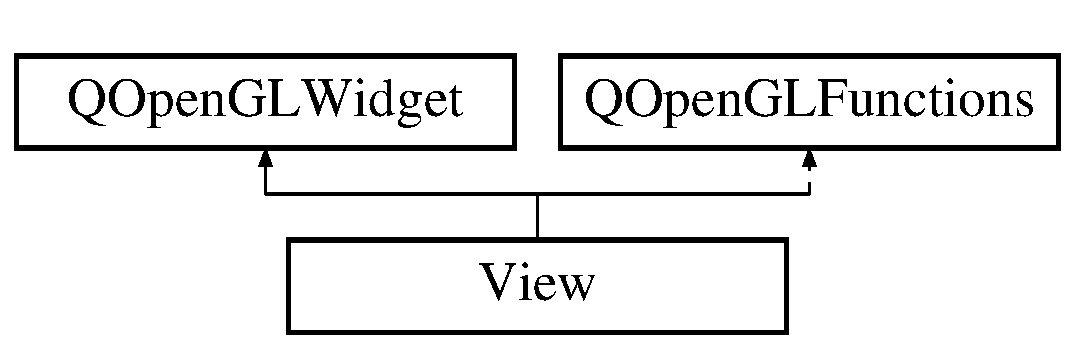
\includegraphics[height=2.000000cm]{class_view}
\end{center}
\end{figure}
\subsection*{Public 成员函数}
\begin{DoxyCompactItemize}
\item 
\hypertarget{class_view_a23bf47b5e5888e35781307cc7507181f}{}\hyperlink{class_view_a23bf47b5e5888e35781307cc7507181f}{View} (\hyperlink{class_model}{Model} $\ast$model, Q\+Widget $\ast$parent=0)\label{class_view_a23bf47b5e5888e35781307cc7507181f}

\begin{DoxyCompactList}\small\item\em A construtor. \end{DoxyCompactList}\item 
\hypertarget{class_view_ad0dc854db9aabbea98a334dec89f785c}{}\hyperlink{class_view_ad0dc854db9aabbea98a334dec89f785c}{$\sim$\+View} ()\label{class_view_ad0dc854db9aabbea98a334dec89f785c}

\begin{DoxyCompactList}\small\item\em A destructor. \end{DoxyCompactList}\item 
void \hyperlink{class_view_a647f520f9b348ce40bfcd9cd1969d3b2}{rotate\+View} (float theta\+X, float theta\+Y, float theta\+Z)
\begin{DoxyCompactList}\small\item\em 旋转视图 \end{DoxyCompactList}\end{DoxyCompactItemize}
\subsection*{Protected 成员函数}
\begin{DoxyCompactItemize}
\item 
\hypertarget{class_view_a30c0d555aa48a2d581238f6e12c500a1}{}void {\bfseries initialize\+G\+L} () Q\+\_\+\+D\+E\+C\+L\+\_\+\+O\+V\+E\+R\+R\+I\+D\+E\label{class_view_a30c0d555aa48a2d581238f6e12c500a1}

\item 
\hypertarget{class_view_af2c68923c2b1775a38529ba49f99877d}{}void {\bfseries resize\+G\+L} (int width, int height) Q\+\_\+\+D\+E\+C\+L\+\_\+\+O\+V\+E\+R\+R\+I\+D\+E\label{class_view_af2c68923c2b1775a38529ba49f99877d}

\item 
\hypertarget{class_view_a4054f0018a33be8db2a2d048e8e79e14}{}void {\bfseries paint\+G\+L} () Q\+\_\+\+D\+E\+C\+L\+\_\+\+O\+V\+E\+R\+R\+I\+D\+E\label{class_view_a4054f0018a33be8db2a2d048e8e79e14}

\item 
\hypertarget{class_view_a1ec6a49f56472d12f37c4a2fccc62392}{}void {\bfseries init\+V\+B\+O} (Q\+Open\+G\+L\+Buffer \&vbo, const Q\+Vector$<$ G\+Lfloat $>$ \&data)\label{class_view_a1ec6a49f56472d12f37c4a2fccc62392}

\item 
\hypertarget{class_view_a918d2a4cd065811dfc7e4e513a1cc3b9}{}Q\+Matrix4x4 {\bfseries paint\+Base} (Q\+Matrix4x4 \&mv\+Matrix)\label{class_view_a918d2a4cd065811dfc7e4e513a1cc3b9}

\item 
\hypertarget{class_view_aaac6dd800eb6b65b9c87260c38633708}{}Q\+Matrix4x4 {\bfseries paint\+Master} (Q\+Matrix4x4 \&mv\+Matrix)\label{class_view_aaac6dd800eb6b65b9c87260c38633708}

\item 
\hypertarget{class_view_acd84d7f155e50a5d4e628f2726053ad3}{}Q\+Matrix4x4 {\bfseries paint\+Assistant} (Q\+Matrix4x4 \&mv\+Matrix)\label{class_view_acd84d7f155e50a5d4e628f2726053ad3}

\item 
\hypertarget{class_view_ab6483d3456cd0b1b49b35012dca4c10d}{}Q\+Matrix4x4 {\bfseries paint\+Bar} (Q\+Matrix4x4 \&mv\+Matrix)\label{class_view_ab6483d3456cd0b1b49b35012dca4c10d}

\end{DoxyCompactItemize}


\subsection{详细描述}
视图类 

\subsection{成员函数说明}
\hypertarget{class_view_a647f520f9b348ce40bfcd9cd1969d3b2}{}\index{View@{View}!rotate\+View@{rotate\+View}}
\index{rotate\+View@{rotate\+View}!View@{View}}
\subsubsection[{rotate\+View}]{\setlength{\rightskip}{0pt plus 5cm}void View\+::rotate\+View (
\begin{DoxyParamCaption}
\item[{float}]{theta\+X, }
\item[{float}]{theta\+Y, }
\item[{float}]{theta\+Z}
\end{DoxyParamCaption}
)\hspace{0.3cm}{\ttfamily [inline]}}\label{class_view_a647f520f9b348ce40bfcd9cd1969d3b2}


旋转视图 


\begin{DoxyParams}{参数}
{\em theta\+X} & 绕x轴角度 \\
\hline
{\em theta\+Y} & 绕y轴角度 \\
\hline
{\em theta\+Z} & 绕z轴角度 \\
\hline
\end{DoxyParams}


该类的文档由以下文件生成\+:\begin{DoxyCompactItemize}
\item 
view.\+h\item 
view.\+cpp\end{DoxyCompactItemize}

%--- End generated contents ---

% Index
\backmatter
\newpage
\phantomsection
\clearemptydoublepage
\addcontentsline{toc}{chapter}{索引}
\printindex

\end{document}
